%!TEX options=--shell-escape
\documentclass[tikz]{standalone}
\usepackage[T1]{fontenc}
\usepackage[utf8]{inputenc}
\usepackage{xcolor}
\usepackage{amsmath}
\usepackage{amssymb}
\usepackage{hyperref}
\usepackage{accsupp}    
\usepackage{graphicx}
\usepackage{mathtools}
\usepackage{pagecolor}
\usepackage{amsmath} % for \dfrac
\usepackage{tikz,ifthen}
\tikzset{>=latex} % for LaTeX arrow head
\usepackage{braket}
\usepackage{pgfplots} 
\usepackage[edges]{forest}
\usetikzlibrary{patterns, backgrounds, arrows.meta}
\setlength{\parindent}{0cm}
\setlength{\parskip}{1em}

\usetikzlibrary{patterns, calc, intersections}

\def\rescale{0.1}
\def\innerwidth{25}
\def\outerwidth{53}
\def\innerlength{35}
\def\trackwidthmax{15}
\def\trackwidthmin{13}
\def\trackarcoffset{1}

\def\delta{2}


\begin{document}
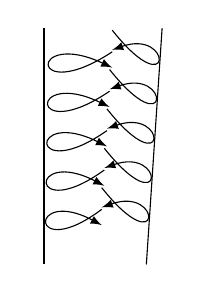
\begin{tikzpicture}[scale=\rescale]


    \draw (0, 0) -- (0, 30);
    \draw (13, 0) -- (15, 30);

\foreach \i in {1, 2, ..., 5} {
      \coordinate (a) at (7 + \i / 3, 5 * \i + 2);
      \coordinate (b) at (7 + \i / 3, 5 * \i);
      \coordinate (bnext) at (7 + \i / 3 + 0.22, 5 * \i - 0.25);



      \path (-2, 5 * \i  + 5) -- (-2, 5 * \i - 5) coordinate(a1);
      \path (-2, 5 * \i - 5) -- (-2, 5 * \i + 5) coordinate(b1);


      \draw[-latex] (a) .. controls (a1) and (b1) .. (b);

      \coordinate (a2) at (7 + \i / 3, 5 * \i + 5 - 0.25);
      \coordinate (b2) at (7 + \i / 3, 5 * \i + 2.25);

      \path (\i /3 + 13, 5 * \i + 5) -- (\i /3 + 14.75, 5 * \i - 5) coordinate(a3);
      \path (\i /3 + 13, 5 * \i - 5) -- (\i /3 + 14.75, 5 * \i + 5) coordinate(b3);

    \draw[-latex] (a2) .. controls (a3) and (b3) .. (b2);

    %\draw (a) -- (b2);
    %\draw (b) -- (bnext);


}

\end{tikzpicture} 
\end{document}

